\documentclass[]{article}
\usepackage{amsmath}
\usepackage{amssymb}
\usepackage{stmaryrd}
\usepackage{latexsym}
\usepackage{graphicx}
\usepackage{fancyhdr}
\usepackage{color}
\usepackage{listings}
\usepackage[top=1in, right=0.75in, left=0.75in]{geometry}
\usepackage[colorlinks=true, linkcolor=blue]{hyperref}

\author{
	Mohammad Hossein Shafizadegan\\
	99104781
}
\title{
	Coding Assignment 3 \\
	Computational Intelligence  \\
	Dr. S. Hajipour
}

\pagestyle{fancy}
\rhead{CI}
\lhead{CHW 3}

\newcommand{\pict}[2]{\begin{center}
		\includegraphics[width=#1\linewidth]{Fig/#2.png}
\end{center}}
\newcommand{\mat}[1]{\begin{bmatrix} #1 \end{bmatrix}}
\newcommand{\deter}[1]{\begin{vmatrix} #1 \end{vmatrix}}

\definecolor{customgreen}{rgb}{0,0.6,0}
\definecolor{customgray}{rgb}{0.5,0.5,0.5}
\definecolor{custommauve}{rgb}{0.6,0,0.8}

\definecolor{dkgreen}{rgb}{0,0.6,0}
\definecolor{gray}{rgb}{0.5,0.5,0.5}
\definecolor{mauve}{rgb}{0.58,0,0.82}

\lstset{frame=tb,
	language=MATLAB,
	aboveskip=3mm,
	belowskip=3mm,
	showstringspaces=false,
	columns=flexible,
	frame=single,	                   % adds a frame around the code
	basicstyle={\small\ttfamily},
	numbers=none,
	numberstyle=\tiny\color{gray},
	keywordstyle=\color{blue},
	commentstyle=\color{dkgreen},
	stringstyle=\color{mauve},
	breaklines=true,
	rulecolor=\color{black},
	breakatwhitespace=true,
	tabsize=3,
	numbers=left,                    % where to put the line-numbers; possible values are (none, left, right)
	numbersep=10pt,                   % how far the line-numbers are from the code
	numberstyle=\tiny\color{customgray}, % the style that is used for the line-numbers
}

\begin{document}
	\begin{figure}
		
\includegraphics[width=0.25\textwidth]{Fig/Sharif.png}
		\centering
	\end{figure}
	\maketitle
	\tableofcontents
	\newpage
		%-----------------------------------------------------------------------------------------------------------------	
	\section{Question 1}
	\subsection{Data visualization}
	After loading the provided data, we separate data corresponding to each class regarding the labels as follows:
	\begin{lstlisting}
		% Separate the data into two classes based on the labels
		class1Data = TrainingData(:, TrainingLabels == 0);
		class2Data = TrainingData(:, TrainingLabels == 1);
	\end{lstlisting}
	Then we visualize the data of each class using built-in function `scatter()`:
	\begin{lstlisting}
		% Plot the data of two classes
		figure;
		scatter(class1Data(1, :), class1Data(2, :), 'ro', 'filled');
		hold on; % Hold on to the current figure
		scatter(class2Data(1, :), class2Data(2, :), 'bo', 'filled');
	\end{lstlisting}
	\pict{0.6}{F1}
	
	\subsection{Train and validation set}
	We randomly separate our data into train and validation set with proportion of 70\% train and 30\% validation. Here is the code used for this section:
	\begin{lstlisting}
		% Split into training and validation sets (70% training, 30% validation)
		[trainInd, valInd, ~] = dividerand(size(TrainingData, 2), 0.7, 0.3, 0);
		trainX = TrainingData(:, trainInd);
		trainY = TrainingLabels(:, trainInd);
		valX = TrainingData(:, valInd);
		valY = TrainingLabels(:, valInd);
	\end{lstlisting} 

	\subsection{Design RBF network with one output neuron}
	In order to implement the RBF network, we are going to use the `newrb()` which is a MATLAB built-in function. In this function the radius of the radial activation function used in the network can be set by calibrating the `spread` input argument.
	\begin{lstlisting}
		% Define the network spec
		hiddenNeurons = 10;
		spread = 1;
		
		% Design the RBF network
		net_1 = newrb(trainX, trainY, 0, spread, hiddenNeurons);
	\end{lstlisting}
	Then we utilize our network to predict the outputs for the validation set and then calculate the accuracy using the following code:
	\begin{lstlisting}
		val_pred_1 = net_1(valX);
		
		% Calculate the classification accuracy
		predictedLabels = round(val_pred_1);
		accuracy = sum(predictedLabels == valY) / numel(valY);
		fprintf('Validation accuracy: %.2f%%\n', accuracy * 100);
	\end{lstlisting}
	\pict{0.4}{F2}
	It can be seen that we have achieved a quite good performance with this value of parameters.
	
	\subsection{Optimal parameters}
	Here we aim to find which value for number of hidden neurons and the radius ($\sigma$) of the activation function, lead to a better outcome. We will check different values of these parameters and plot the accuracy regarding to these parameters. Here is the code:
	\begin{lstlisting}
		nhidden = 1:20;
		sigma = 0.1:0.1:10;
		[X, Y] = meshgrid(nhidden, sigma);
		
		acc = zeros(length(nhidden), length(sigma));
		for i=1:length(nhidden)
			for j=1:length(sigma)
				acc(i,j) = pred_RBF_1out(nhidden(i), sigma(j), valX, valY, trainX, trainY);
			end
		end
	\end{lstlisting}
	Now we print the spec resulted into the the best accuracy using the following code:
	\begin{lstlisting}
		[~, idx] = max(acc(:));
		[row, col] = ind2sub(size(acc), idx);
		
		fprintf('Best accuracy of %f achieved with nhidden = %d and sigma = %f \n', ...
			   		acc(row, col), nhidden(row), sigma(col));
	\end{lstlisting}
	\pict{0.7}{F5}
	It can be seen that the best choice for number of hidden neurons is 19 and the best choice for radius is 2.\\\\
	Now we plot the 3D curve, demonstrating the value of accuracy for different values of radius and number of hidden neurons.
	\begin{center}
		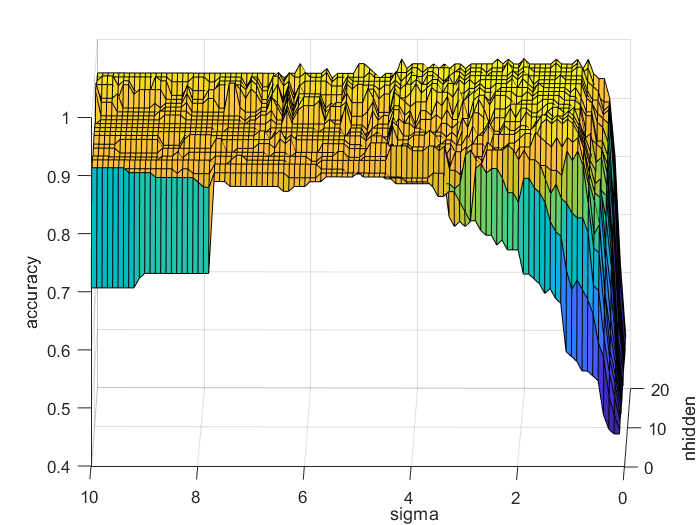
\includegraphics[width=0.4\linewidth]{Fig/F3.png}
		\qquad\qquad
		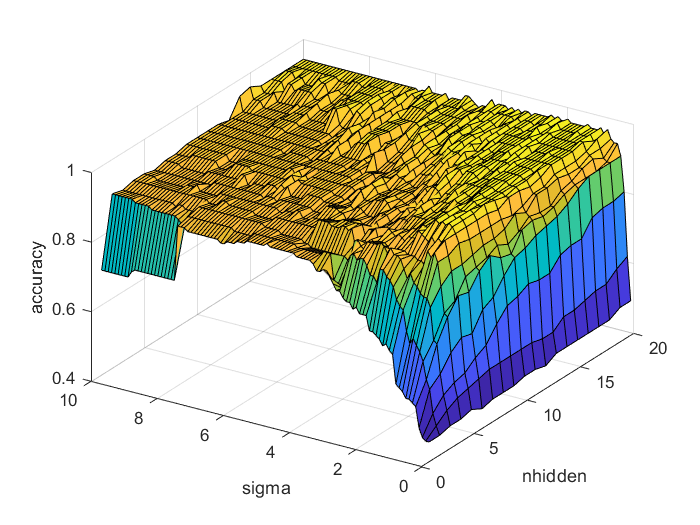
\includegraphics[width=0.4\linewidth]{Fig/F4.png}
	\end{center}
	
	\subsection{RBF network with two output neurons}
	In order to design our network, we have to perform some modifications. The network will have two output neurons. We assume that the first output neuron indicates the probability of belonging to the first class and in a same way, the second output neuron will indicate the probability of a sample to belong to the second class (label).\\\\
	Regarding this, we will modify the output for train and validation set as follows:
	\begin{lstlisting}
		train_Y_2 = [1-trainY; trainY];
		val_Y_2 = [1-valY; valY]; 
	\end{lstlisting}
	Finally in order to decide the label of a sample, we assign them the class with higher probability. This can be done as follows:
	\begin{lstlisting}
		hiddenNeurons = 20;
		% Design the RBF network
		net_2 = newrb(trainX, train_Y_2, 0, 1, hiddenNeurons);
		
		val_Y_2 = [1-valY; valY];
		val_pred_2 = sim(net_2, valX);
		
		% Calculate the classification accuracy
		[~, predictedLabels] = max(val_pred_2);
		[~, actualLabels] = max(val_Y_2);
	\end{lstlisting}
	Now we assess our model:
	\pict{0.7}{F6}
	In order to observe how number of hidden neurons and value of radius affect this network, we pursue the same approach as we did for the previous network:
	\pict{0.8}{F7}
	\begin{center}
		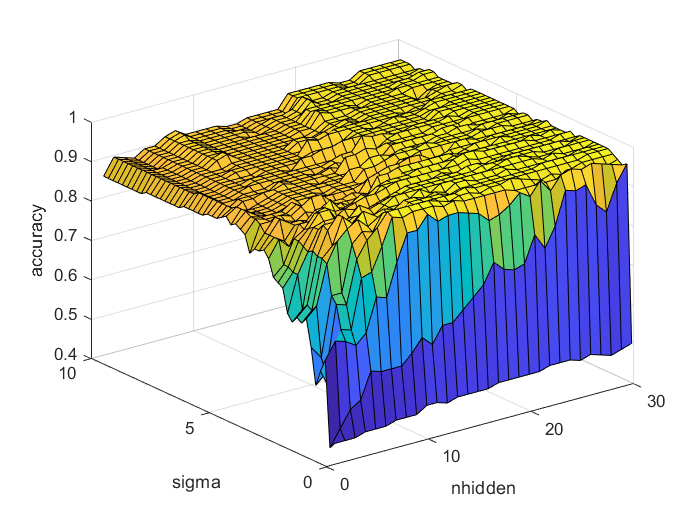
\includegraphics[width=0.4\linewidth]{Fig/F8.png}
		\qquad\qquad
		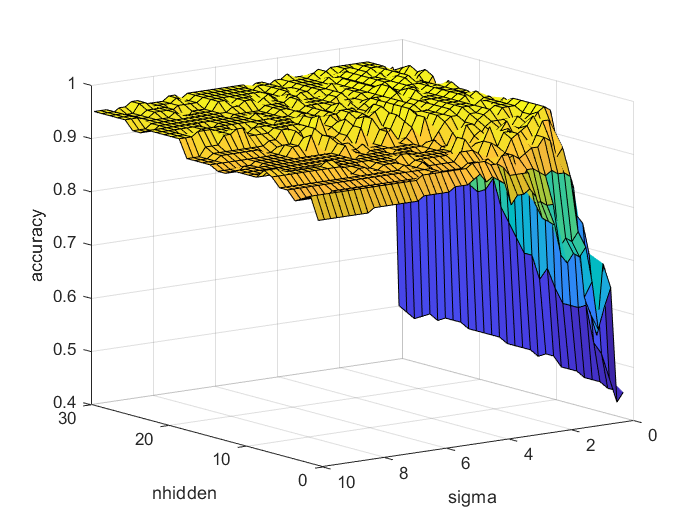
\includegraphics[width=0.4\linewidth]{Fig/F9.png}
	\end{center}

		%-----------------------------------------------------------------------------------------------------------------	
	\section{Question 2}
	\subsection{Part 1}
	We have developed a function called `my\_kmeans`. It takes input data, the number of clusters (k), and initial centroids. The code iteratively assigns data points to the nearest centroids and updates the centroid positions until convergence is reached. It does this by calculating distances between data points and centroids, assigning labels to each data point based on the nearest centroid, and updating the centroids based on the mean of the data points assigned to each cluster. The process continues until the centroids no longer change.\\\\
	The function then returns the resulting centroids and labels. Overall, it's a simple implementation of k-means clustering, performing iterative assignments and updates to find cluster centers and assign data points to clusters.
	\begin{lstlisting}
		% Initialize labels and previous centroids
		labels = zeros(size(data, 2), 1);
		prevCentroids = zeros(size(centroids));
		
		% Iterate until convergence
		while ~isequal(centroids, prevCentroids)
			
			% Assign each data point to the nearest centroid
			for i = 1:size(data, 2)
				distances = sum((data(:, i) - centroids).^2, 1);  % Adjusted indexing
				[~, index] = min(distances);
				labels(i) = index;
			end
			
			% Update the centroids
			prevCentroids = centroids;
			for j = 1:k
				clusterPoints = data(:, labels == j);
				centroids(:, j) = mean(clusterPoints, 2);  % Adjusted mean calculation
			end
		end
	\end{lstlisting}
	Now we assess the performance of our function for dividing data into 5 clusters. Using the following code we will visualize the results:
	\begin{lstlisting}
		hold on;
		colors = lines(k);
		for i = 1:k
			clusterPoints = DataNew(:, labels == i);
			scatter(clusterPoints(1, :), clusterPoints(2, :), [], colors(i, :), 'filled');
		end
		scatter(centroids(1, :), centroids(2, :), 100, 'k', 'filled');
		hold off;
		title('k-means Clustering');
	\end{lstlisting}
	\pict{0.6}{F10}
	
	\subsection{Part 2}
	Here we check the results for 4 and 6 clusters below:
	\begin{center}
		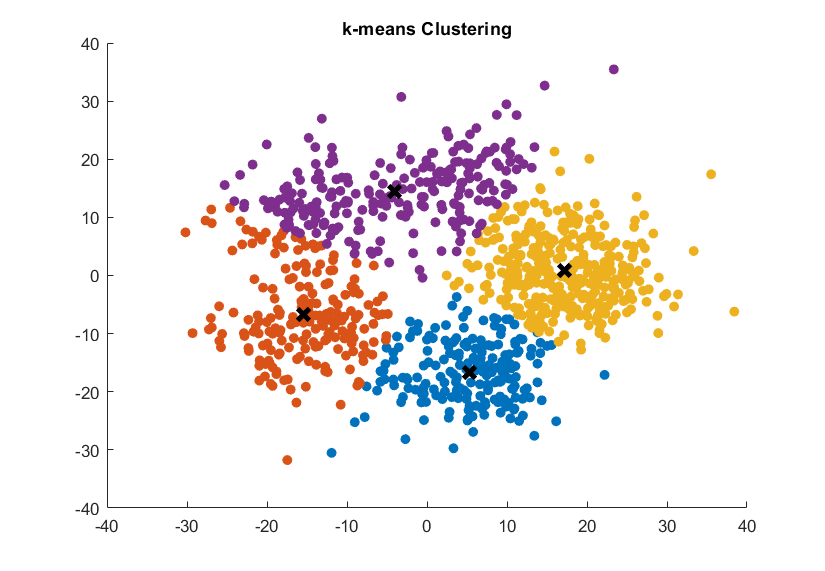
\includegraphics[width=0.45\linewidth]{Fig/F11.png}
		\qquad\qquad
		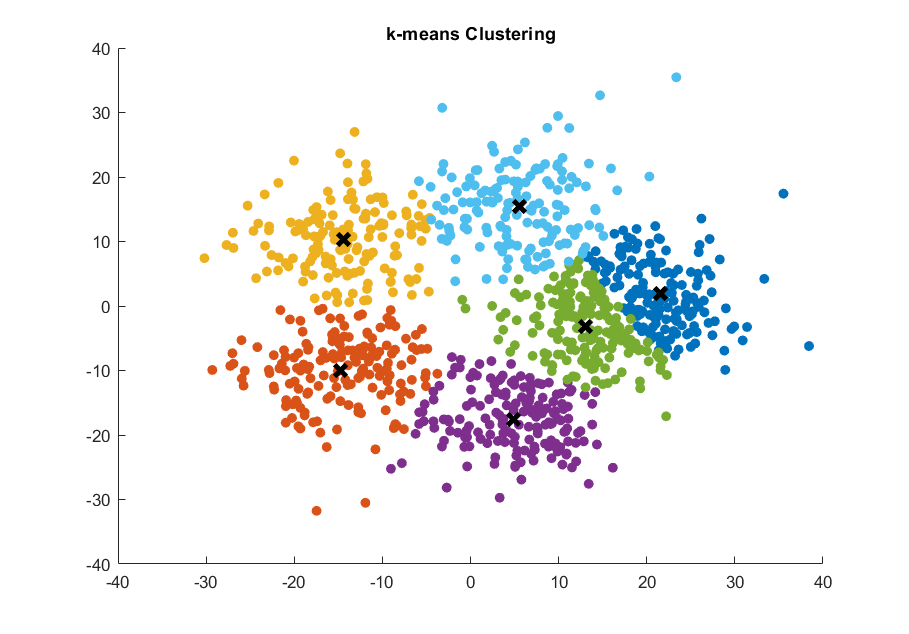
\includegraphics[width=0.45\linewidth]{Fig/F12.png}
	\end{center}
	
	\subsection{MATLAB kmeans}
	Now we use the MATLAB builtin function as follows:
	\begin{lstlisting}
		k=6;
		[labels, centroids] = kmeans(DataNew', k);
		plot_clusters(k, DataNew, centroids', labels)
	\end{lstlisting}

	\begin{center}
		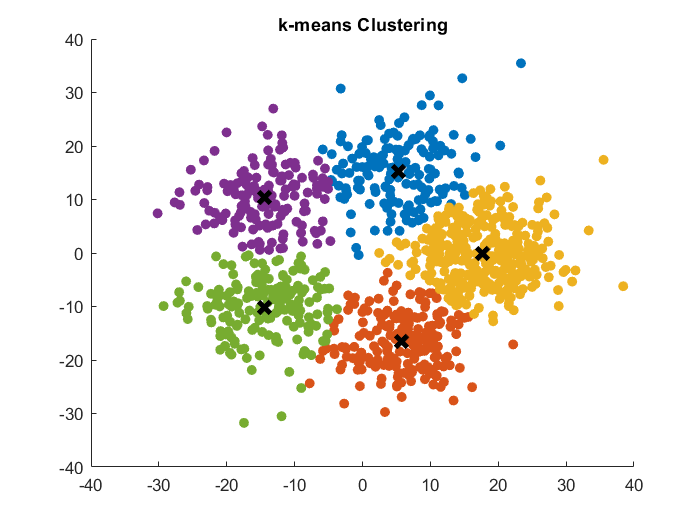
\includegraphics[width=0.3\linewidth]{Fig/F13.png}
		\qquad
		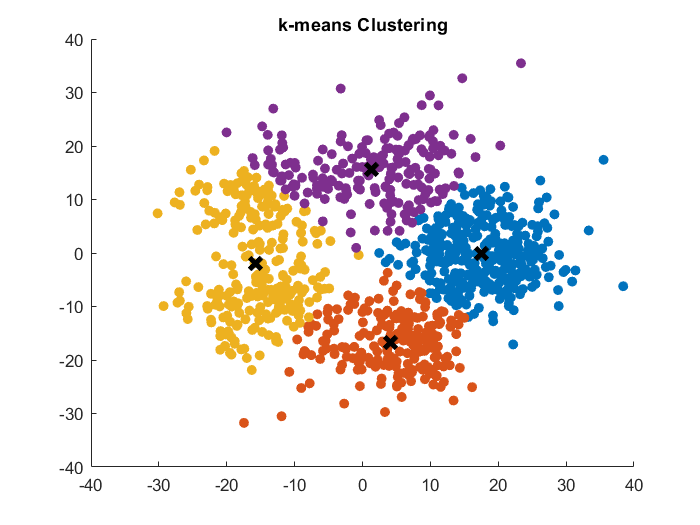
\includegraphics[width=0.3\linewidth]{Fig/F14.png}
		\qquad
		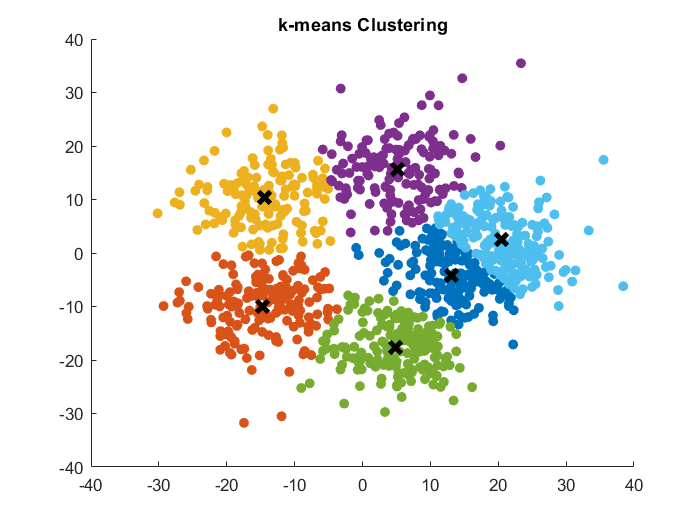
\includegraphics[width=0.3\linewidth]{Fig/F15.png}
	\end{center}

	\subsection{Hierarchical clustering}
	Hierarchical clustering is a machine learning algorithm used to group unlabeled datasets into a tree-shaped structure called a dendrogram. It is an unsupervised learning method that starts by treating each data point as a separate cluster and then iteratively combines the closest clusters until a stopping criterion is reached. The algorithm can be divided into two approaches: Agglomerative and Divisive. The Agglomerative approach is a bottom-up approach, in which the algorithm starts with taking all data points as single clusters and merging them until one cluster is left. The Divisive algorithm is the reverse of the Agglomerative algorithm as it is a top-down approach.\\\\
	Hierarchical clustering is useful when we don’t have knowledge about the predefined number of clusters. It is also helpful when we want to create clusters of different sizes.	We have implement this method in MATLAB using the following code for 5 clusters:
	\begin{lstlisting}
		%Perform hierarchical clustering
		linkageMatrix = linkage(data, 'ward', 'euclidean'); 
		
		% Plot the dendrogram
		dendrogram(linkageMatrix);
		
		k = 5; % Specify the desired number of clusters
		clusterLabels = cluster(linkageMatrix, 'maxclust', k);
		plot_clusters_2(k, data', clusterLabels);
		
	\end{lstlisting}
	Here are the results:
	\pict{0.4}{F17}
	\pict{0.7}{F16}
	Also we will generate the results for 4 and 6 clusters:
	\begin{center}
		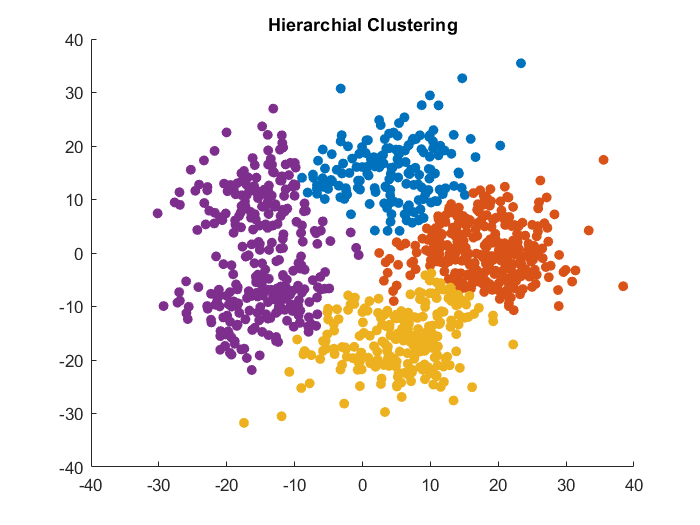
\includegraphics[width=0.45\linewidth]{Fig/F18.png}
		\qquad
		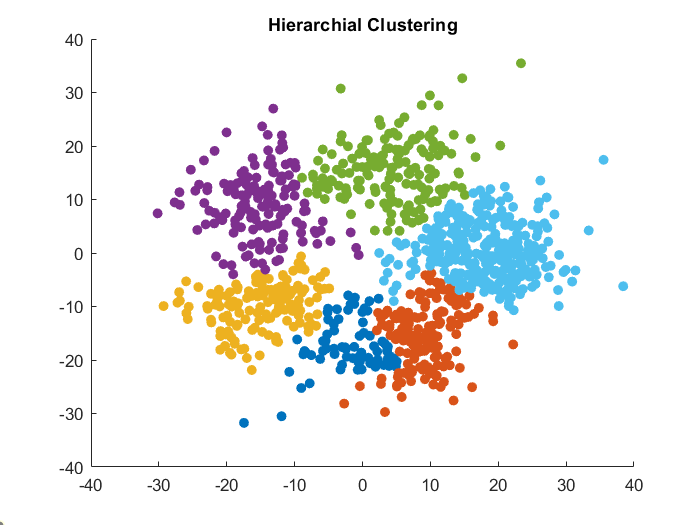
\includegraphics[width=0.45\linewidth]{Fig/F19.png}
	\end{center}

		%-----------------------------------------------------------------------------------------------------------------	
	\section{Question 3}
	\subsection{Genetic Algorithm}
	First we simply load the data. Then we define the lower and upper bound of the centroid of the clusters regarding the minimum and maximum value of data. After that using MATLAB built-in function called `optimoptions()`, we define the genetic algorithm options as follows:
	\begin{lstlisting}
		% Define the genetic algorithm options
		options = optimoptions('ga', 'Display', 'iter', 'MaxGenerations', 100, 'PopulationSize', 50);
	\end{lstlisting}
	The next step is to define the fitness function regarding the problem of kmeans. The following function is developed to do so:
	\begin{lstlisting}
		function fitness = kmeansFitness(data, centroids, K)
			% Reshape the centroids
			centroids = reshape(centroids, K, []);
			
			% Compute distances from each data point to each centroid
			distances = pdist2(data, centroids);
			
			% Find the closest centroid for each data point
			[~, idx] = min(distances, [], 2);
			
			% Compute the sum of squared distances
			fitness = sum(sum((data - centroids(idx, :)).^2));
		end
	\end{lstlisting}
	Then we run the genetic algorithm using the builtin function `ga()` as follows:
	\begin{lstlisting}
		% Run the genetic algorithm
		centroidsGA = ga(fitnessFunction, size(data, 2) * K, [], [], [], [], lb, ub, [], options);
	\end{lstlisting} 
	Now we have the final and resulting positions of the centroids. In order to visualize the results we have to find the nearest data points to these clusters and plot the results. The following code will do this:
	\begin{lstlisting}
		% Compute distances from each data point to each centroid
		distancesGA = pdist2(data, centroidsGA);
		
		% Find the closest centroid for each data point
		[~, idxGA] = min(distancesGA, [], 2);
		
		% Visualize the results
		figure;
		scatter(data(:, 1), data(:, 2), 30, idxGA, 'filled');
		hold on;
		scatter(centroidsGA(:, 1), centroidsGA(:, 2), 100, 'k', 'x', 'LineWidth', 2);
		title('Clusters with Optimized Centroids');
		xlabel('Feature 1');
		ylabel('Feature 2');
		colormap(gca, jet(K));
		
	\end{lstlisting}
	\pict{0.4}{F20}
	
	\subsection{PSO}
	In this section, we first sets up the k-means parameters, including the number of clusters and the data to be clustered.
	\begin{lstlisting}
		% Set up PSO parameters
		options = optimoptions('particleswarm', 'SwarmSize', 50, 'MaxIterations', 100);
	\end{lstlisting}
	In this algorithm, each particle consists of an array with 10 ($2 \times k$) elements, indicating the position of the desired 5 (k in general) centroids. Regarding this particle presentation we run the PSO algorithm using the following code:
	\begin{lstlisting}
		% Run PSO to find cluster centroids
		numVariables = k * size(data, 2);
		lb = repelem(min(data), k);
		ub = repelem(max(data), k);
		
		[bestPositions, cost] = particleswarm(objectiveFunction, numVariables, lb, ub, options);
	\end{lstlisting}
	The final cluster centroids are obtained by reshaping the best positions, and the data points are assigned to the final centroids.
	\begin{lstlisting}
		% Reshape the best positions to get the final cluster centroids
		numElementsPerCluster = numVariables / k;
		bestCentroids = reshape(bestPositions(1 : floor(numElementsPerCluster) * k), k, []);
		
		% Assign data points to the final centroids
		[~, clusterIndices] = pdist2(bestCentroids, data, 'euclidean', 'Smallest', 1);
	\end{lstlisting}
	\pict{0.4}{F21}
	
	\subsection{ACO}
	First we set parameters such as the number of clusters, ants, and maximum iterations. Then we simply load our data.\\\\
	We have developed the `antColonyClustering` function which implements the ACO algorithm. Here are the things we have considered in developing this function:
	\begin{itemize}
		\item Initializes pheromones.
		\item Runs the main loop for a specified number of iterations.
		\item Constructs solutions for each ant using the `constructSolution` function.
		\item Updates pheromones based on the solutions using the `updatePheromones` function.
		\item Evaluates the solutions and finds the best solution with the lowest sum of squared distances.
	\end{itemize}
	Here is the code:
	\begin{lstlisting}
		% Main loop
		for iteration = 1:maxIterations
			solutions = zeros(numAnts, size(data, 1));
			
			% Ant solutions construction
			for ant = 1:numAnts
				solutions(ant, :) = constructSolution(pheromones);
			end
			
			% Pheromone update
			pheromones = updatePheromones(pheromones, solutions, data);
			
			% Find the best solution
			[minDistance, minIndex] = min(evaluateSolutions(solutions, data));
			bestSolution = solutions(minIndex, :);
			bestCentroids = calculateCentroids(data, bestSolution, numClusters);
			
		end
	\end{lstlisting}
	Using the `constructSolution` function, we construct a solution for each data point by probabilistically assigning it to a cluster based on pheromones.
	\begin{lstlisting}
		function solution = constructSolution(pheromones)
			% Construct a solution using pheromones for k-means clustering
			
			numDataPoints = size(pheromones, 1);
			
			% Initialize probabilities for each data point to be assigned to each cluster
			probabilities = pheromones;
			
			% Normalize probabilities
			probabilities = probabilities ./ sum(probabilities, 2);
			
			% Assign each data point to a cluster based on probabilities
			solution = zeros(1, numDataPoints);
			for point = 1:numDataPoints
				solution(point) = selectCluster(probabilities(point, :));
			end
		end
	\end{lstlisting}
	We evaluate the quality of solutions based on the sum of squared distances between data points and their assigned cluster centroids.\\\\
	We have developed the `updatePheromones` function to implement the updating procedure of the pheromones. This function:
	\begin{itemize}
		\item Updates pheromones based on the assigned clusters in each solution.
		\item Uses an evaporation rate to decay existing pheromones and a deposit rate to add new pheromones based on the inverse of the squared distance.
	\end{itemize}
	\begin{lstlisting}
		function newPheromones = updatePheromones(pheromones, solutions, data)
			% Update pheromones based on the assigned clusters
			evaporationRate = 0.05;
			depositRate = 0.8;
			
			% Evaporation
			pheromones = (1 - evaporationRate) * pheromones;
			
			for ant = 1:size(solutions, 1)
				centroids = calculateCentroids(data, solutions(ant, :), max(solutions(ant, :)));
				
				for point = 1:size(data, 1)
					cluster = solutions(ant, point);
					temp = min(norm(data(point, :) - centroids(cluster, :))^2);
					pheromones(point, cluster) = pheromones(point, cluster) + 10 * depositRate / temp;
				end
			end
			
			% Normalize pheromones
			newPheromones = pheromones ./ sum(pheromones, 2);
		end
	\end{lstlisting}
	
	Finally we assess our code for the provided data and visualize the results:
	\pict{0.5}{F22}
\end{document}